% Template latex non officiel pour rapport de TP EEA.
% C'est un template pour thèse que j'ai adapté et 
% auquel j'ai ajouté des éléments au fil du temps pour mes rapports de TP.
% En cas de problèmes n'hésites pas a me contacter.
% David Tocaven
% david.tocaven@gmail.com


%%% /!\ /!\ /!\ /!\ /!\ /!\
% Se compile avec PDFLatex
%%% /!\ /!\ /!\ /!\ /!\ /!\
%%=================================================%%
%%						MAIN
%%=================================================%%


\documentclass[a4paper]{report}

%====================== PACKAGES ======================
\usepackage{bbold}
\usepackage{soul}				% souligner
\usepackage{dsfont}
\usepackage[french]{babel}		% Pour avoir le document en français
\usepackage[utf8x]{inputenc}	% Encodage du document
\usepackage{float}				% Pour gérer les positionnement d'images
\usepackage{amsmath}
\usepackage{mathrsfs}			% Pour les lettres calligraphiques équation
\usepackage{url}				% Pour faire des hyperliens vers le web
\usepackage{color}
% pour les informations sur un document compilé en PDF et les liens externes / internes
\usepackage{hyperref}			% Pour faire des hyperliens
\usepackage{array}				% Pour faire des tableaux
\usepackage{tabularx}
% pour utiliser 		% floatbarrier
%\usepackage{placeins}
%\usepackage{floatrow}
\usepackage{setspace}			% Espacement entre les lignes
\usepackage{abstract}			% Modifier la mise en page de l'abstract
\usepackage[T1]{fontenc}		% Police et mise en page (marges) du document
\usepackage[top=2cm, bottom=2cm, left=2cm, right=2cm]{geometry}
\usepackage{pdfpages}			% pour inclures des pdf comme des images
\usepackage{subfig}				% Pour les galerie d'images
\usepackage{listings}			% pour inclure du code dans le doc
\usepackage{soul}				% Pour surligner
\usepackage{enumitem}

\sethlcolor{grisclair}
\definecolor{darkgreen}{RGB}{0,100,0}

% Import from other TP
\usepackage{titlesec, blindtext, color}	
\definecolor{gray75}{gray}{0.75}
\newcommand{\hsp}{\hspace{20pt}}
\titleformat{\chapter}[hang]{\Huge\bfseries}{\thechapter\hsp\textcolor{gray75}{|}\hsp}{0pt}{\Huge\bfseries}

%====================== INFORMATION ET REGLES ======================

%rajouter les numérotation pour les \paragraphe et \subparagraphe
\setcounter{secnumdepth}{4}
\setcounter{tocdepth}{4}

\hypersetup{							% Information sur le document
pdfauthor = { NOM },				% Auteurs
pdftitle = {Matière - Titre - Sujet },		% Titre du document
pdfsubject = {matière},		% Sujet
pdfkeywords = {},				% Mots-clefs
pdfstartview={FitH}}					% ajuste la page à la largueur de l'écran
%pdfcreator = {MikTeX},% Logiciel qui a crée le document
%pdfproducer = {}} % Société avec produit le logiciel

\newcounter{cpt1}						% Compteur pour les n° de ligne dans les prog de l'annexe1
\newcommand\increm{\arabic{cpt1}\addtocounter{cpt1}{1}}
%initialisation de l'intégrateur de language C



%======================== DEBUT DU DOCUMENT ========================

\begin{document}

%\lstset{
%  language=C,                	  % choose the language of the code
%  numbers=left,                   % where to put the line-numbers
%  stepnumber=1,                   % the step between two line-numbers.
%  numbersep=5pt,                  % how far the line-numbers are from the code
%  backgroundcolor=\color{white},  % choose the background color. You must add \usepackage{color}
%  showspaces=false,               % show spaces adding particular underscores
%  showstringspaces=false,         % underline spaces within strings
%  showtabs=false,                 % show tabs within strings adding particular underscores
%  tabsize=2,                      % sets default tabsize to 2 spaces
%  captionpos=b,                   % sets the caption-position to bottom
%  breaklines=true,                % sets automatic line breaking
%  breakatwhitespace=true,         % sets if automatic breaks should only happen at whitespace
%  title=\lstname,                 % show the filename of files included with \lstinputlisting;
%}
%régler l'espacement entre les lignes
\newcommand{\HRule}{\rule{\linewidth}{0.5mm}}


%page de garde
%%=================================================%%
%%						TITRE DU DOCUMENT (1 PAGE)
%							  Pas totalement fini
%%=================================================%%

\begin{titlepage}
\begin{center}

% Upper part of the page. The '~' is needed because only works if a paragraph has started.


\includegraphics[width=0.60\textwidth]{./page_de_garde/logo_ups.png}~\\[1cm]

\textsc{\LARGE Université Paul Sabatier}\\[1.5cm]

\textsc{\Large \bf Modèle Temporel avancé }\\[0.5cm]

% Title
\HRule \\[0.4cm]

{\huge \bfseries  - TP : \textsc{Système de Traitement Automatisé} -}

\HRule \\[1.5cm]

% Author and supervisor
\begin{minipage}{0.4\textwidth}
\begin{flushleft} \large
\emph{Auteurs:}\\
Lucien \textsc{Rakotomalala}\\
David \textsc{Tocaven}\\
\end{flushleft}
\end{minipage}
\begin{minipage}{0.58\textwidth}
\begin{flushright} \large
\emph{Encadrant:} \\
\textbf{ Pauline \textsc{Ribot}}\\
\textbf{ Euriell \textsc{Le Corronc}}\\
\textbf{ Michel \textsc{Combacau}}
\end{flushright}
\end{minipage}
\newline
\newline
\vfill
% une éventuelle image
\fbox{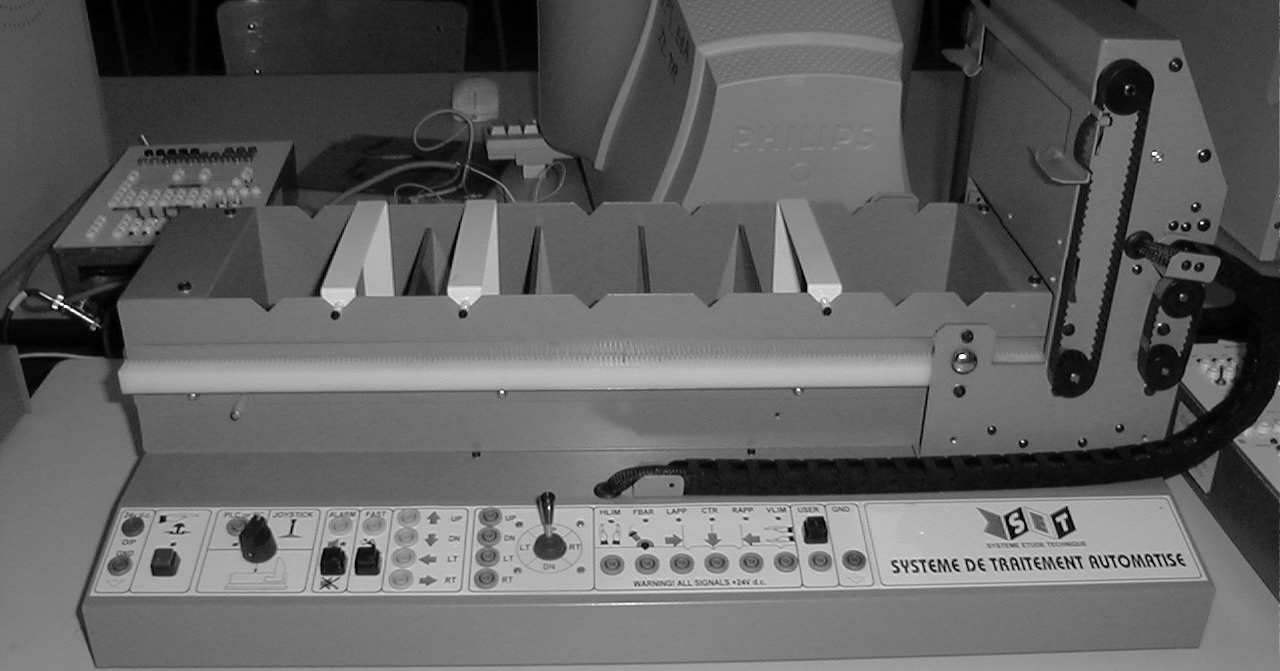
\includegraphics[width=.6\textwidth]{./page_de_garde/M2ASTR-TP-MACSED-STA.jpg}}~\\[1cm]

\vfill
% logo fsi & eea
\begin{tabular}{cc}
   
\includegraphics[height=2cm]{./page_de_garde/logo_fsi.png} \hspace{2cm} &
    \hspace{2cm}
   
\includegraphics[height=2cm]{./page_de_garde/logo_eea.jpg} \\
\end{tabular}

% Bottom of the page
{\large \today}

\end{center}
\end{titlepage}
	

%page blanche
\newpage
~
\tableofcontents
\thispagestyle{empty}
\setcounter{page}{0}
%ne pas numéroter le sommaire


%espacement entre les lignes d'un tableau
\renewcommand{\arraystretch}{1.5}

%====================== INCLUSION DES PARTIES ======================
%
%~
\thispagestyle{empty}
%recommencer la numérotation des pages à "1"
\setcounter{page}{0}

\chapter*{Introduction}
\addcontentsline{toc}{chapter}{Introduction}
\label{chap:Intro}	% Importation de introduction.tex

\chapter{Modélisation et analyse de la réalisation d'une opération}\label{chap:realisationUneOperation}
Nous allons dans un premier temps réaliser une modélisation par réseau de Petri temporel de la réalisation d'une opération. Cette modélisation sera générique à la réalisation de toute opération $O_i$. Ensuite, nous réaliserons un code C qui permet d'estimer les durées des différentes opérations. Finalement, nous analyserons le réseau de Petri à l'aide de \emph{TINA 2.8.4}.

\section{Modèle réseau de Petri temporel d'une opération}
Nous avons, pour modélisation générique d'une opération, considéré que le chariot de déplacement se trouve en bas. Voici le réseau de Petri temporel (voir figure \ref{fig:RdPTempo_generique}) : \\
\begin{figure}[!ht]
\centering
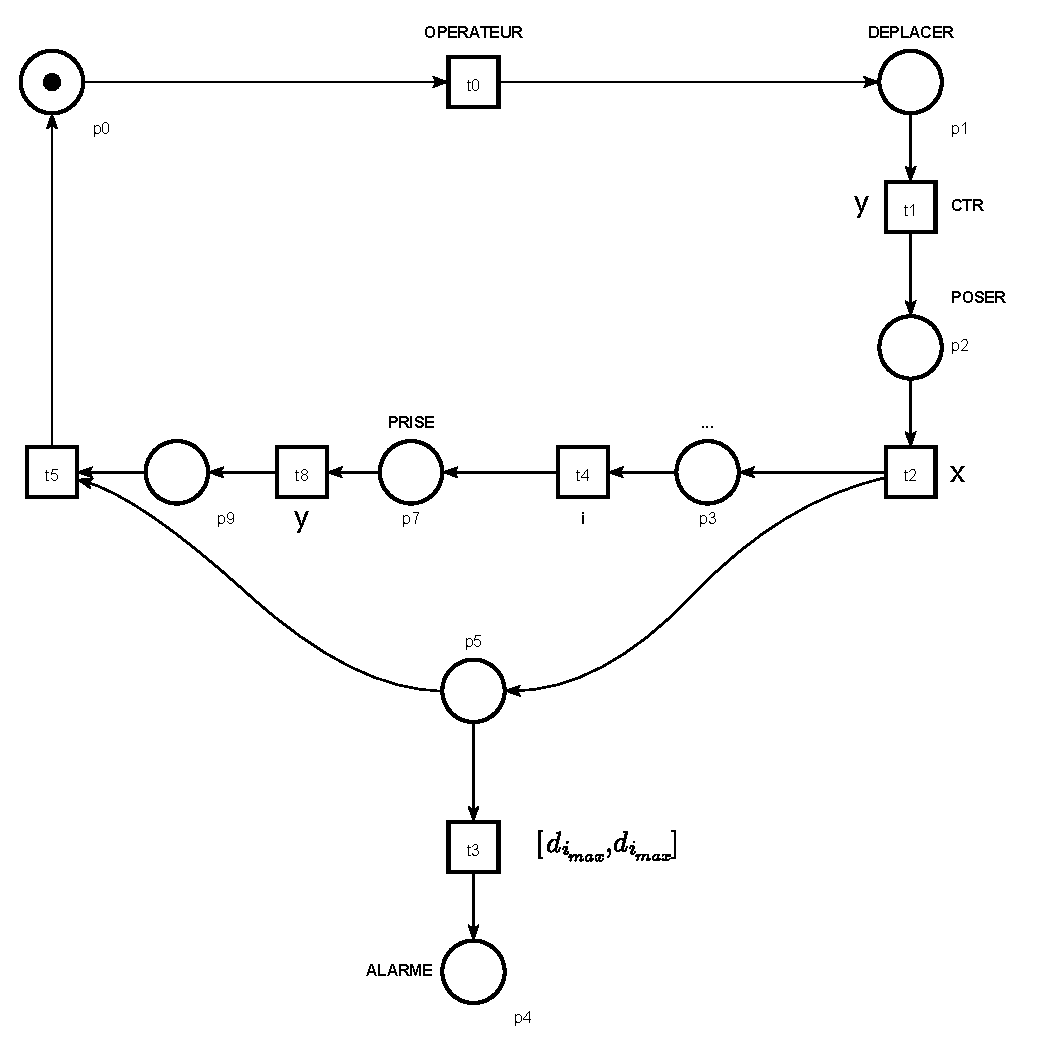
\includegraphics[width=.57\textwidth]{./I/images/III-1_v3.pdf}
\caption{\label{fig:RdPTempo_generique}Modèle réseau de Petri générique d'une opération.}
\end{figure}


Nous considérerons que l'action \emph{DEPLACER()} et l'événement \emph{FinDeplacer} correspondent à, respectivement, \emph{AVANCER()} et \emph{FinAvancer} si le chariot est à droite de l'emplacement de l'opération $o_i$  ou \emph{RECULER()} et \emph{FinReculer} si celui-ci est à gauche.


Le marquage initial est constitué d'un unique jeton sur la place $p_0$. Ce jeton, une fois que la transition $t_0$ est sensibilisée et tirée (pour cela il faut que l'événement \emph{OPERATEUR()} est eu lieu), est en $p_1$. Le chariot se déplace tant qu'il y a un jeton en $p_1$. Le jeton reste en $p_1$ jusqu'à ce que le charriot arrive à destination, c'est-à-dire que \emph{FinDeplacer} se déclenche. Lorsque cet événement ce produit, la transition $t_1$ est sensibilisée et tirée (le déplacement prend un temps $y$ qui est représenté sur la transition $t_1$). Ensuite, un jeton marque la place $p_2$ ce qui déclenche l'action \emph{POSER()}. Cette action prend un temps $x$ et celui-ci est représenté sur la transition $t_2$. Une fois le temps $x$ écoulé, la transition $t_2$ est tiré et les places $p_3$ et $p_6$ sont marqués d'un jeton chacun. 

À partir de cet état, il y a deux jetons dans le réseau : un permet de décrire le comportement du chariot et un autre, celui qui marque $p_6$, permet de déclencher l'alarme si la pièce qui subit l'opération $o_i$ n'est pas reprise avant le temps maximal de l'opération.  En effet, le jeton présent en $p_6$, au bout d'un temps $d_{i_{max}}$, va être consommé par la transition $t_6$ et un jeton va marquer $p_7$. Ceci déclenchera l'action \emph{ALARME()}.
Il faut donc que le jeton présent en $p_3$ arrive en $p_5$ en moins de $d_{i_{max}}$ unités de temps pour que l'alarme ne se déclenche pas. De cette façon, le tir de la transition $t_5$, qui nécessite et consomme un jeton en $p_6$ et un jeton en $p_5$, empêchera l'alarme de sonner et permettra d'effectuer une nouvelle opération (retour au marquage initial). 
La place $p_3$ à un événement \emph{...}, cela représente la possibilité d'effectuer n'importe(s) quelle(s) action(s) et de revenir à l'emplacement de l'opération $o_i$, de façon à ce que l'action en $p_4$, \emph{PRISE()}, de durée $y$, permette de récupérer la pièce. La transition $t_3$ est marquée de la temporisation $i$. Celle-ci représente le temps de(s) action(s) de la place $p_4$ et/ou un temps d'attente afin que l'on récupère la pièce à la fin de l'opération $ç_i$. Ainsi, si l'on souhaite que l'alarme ne sonne pas, il faut que $i + y < d_{i_{max}}$.

\section{Estimation de Prise/Pose et Avance/Recule}
\begin{center}
\textit{Voir annexe \ref{Annex:MesuresXY}, page \pageref{Annex:MesuresXY}.}
\end{center}
Nous avons maintenant besoin d'identifier le temps de \emph{AVANCER()} (égal à celui de \emph{RECULER()}) que l'on appelait précédemment$y$  et de \emph{PRISE()} (équivalent à celui de \emph{POSE()}) appelait $y$. Pour cela, nous avons créer, à partir d'un code fourni, un code permettant de mesurer les temps $x$ et $y$. Pour mesurer le temps d'une action, nous avons stocké le temps du PC à l'instant du début de l'action, puis nous avons stocké le temps à la fin de celle-ci et avons affiché la soustraction des deux temps sur le terminal. 
Nous avons déterminé que :
\begin{eqnarray}
x &=& \begin{bmatrix}
1 & 1
\end{bmatrix} \text{seconde}\\
y &=& \begin{bmatrix}
3 & 3
\end{bmatrix} \text{secondes}\\
\end{eqnarray}
\section{Analyse du modèle}
Grâce aux mesures précédentes, nous avons pus remplacer $x$ et $y$ par des valeurs temporelles sur le modèle générique. Nous avons choisi arbitrairement les valeurs de $d_{i_{min}} = 13$ secondes et $d_{i_{max}} = 16$ secondes, respectivement le temps minimal de l'opération et le temps maximal de l'opération $o_i$.  Ainsi, nous avons la condition suivante qui doit être respectée $i <d_{i_{max}}-y$, soit $i < 13$ secondes. Donc il "reste" moins de 13 secondes afin de réaliser d'autres opérations. Nous allons fixer une temporisation  $i=\begin{bmatrix}
12& 12
\end{bmatrix}$ secondes pour étudier le réseau. 

Figure \ref{fig:RdPTempo_generique_indentif}, voici le nouveau réseau de Petri temporel.
\begin{figure}[!ht]
\begin{minipage}[t]{.4\textwidth}
\centering
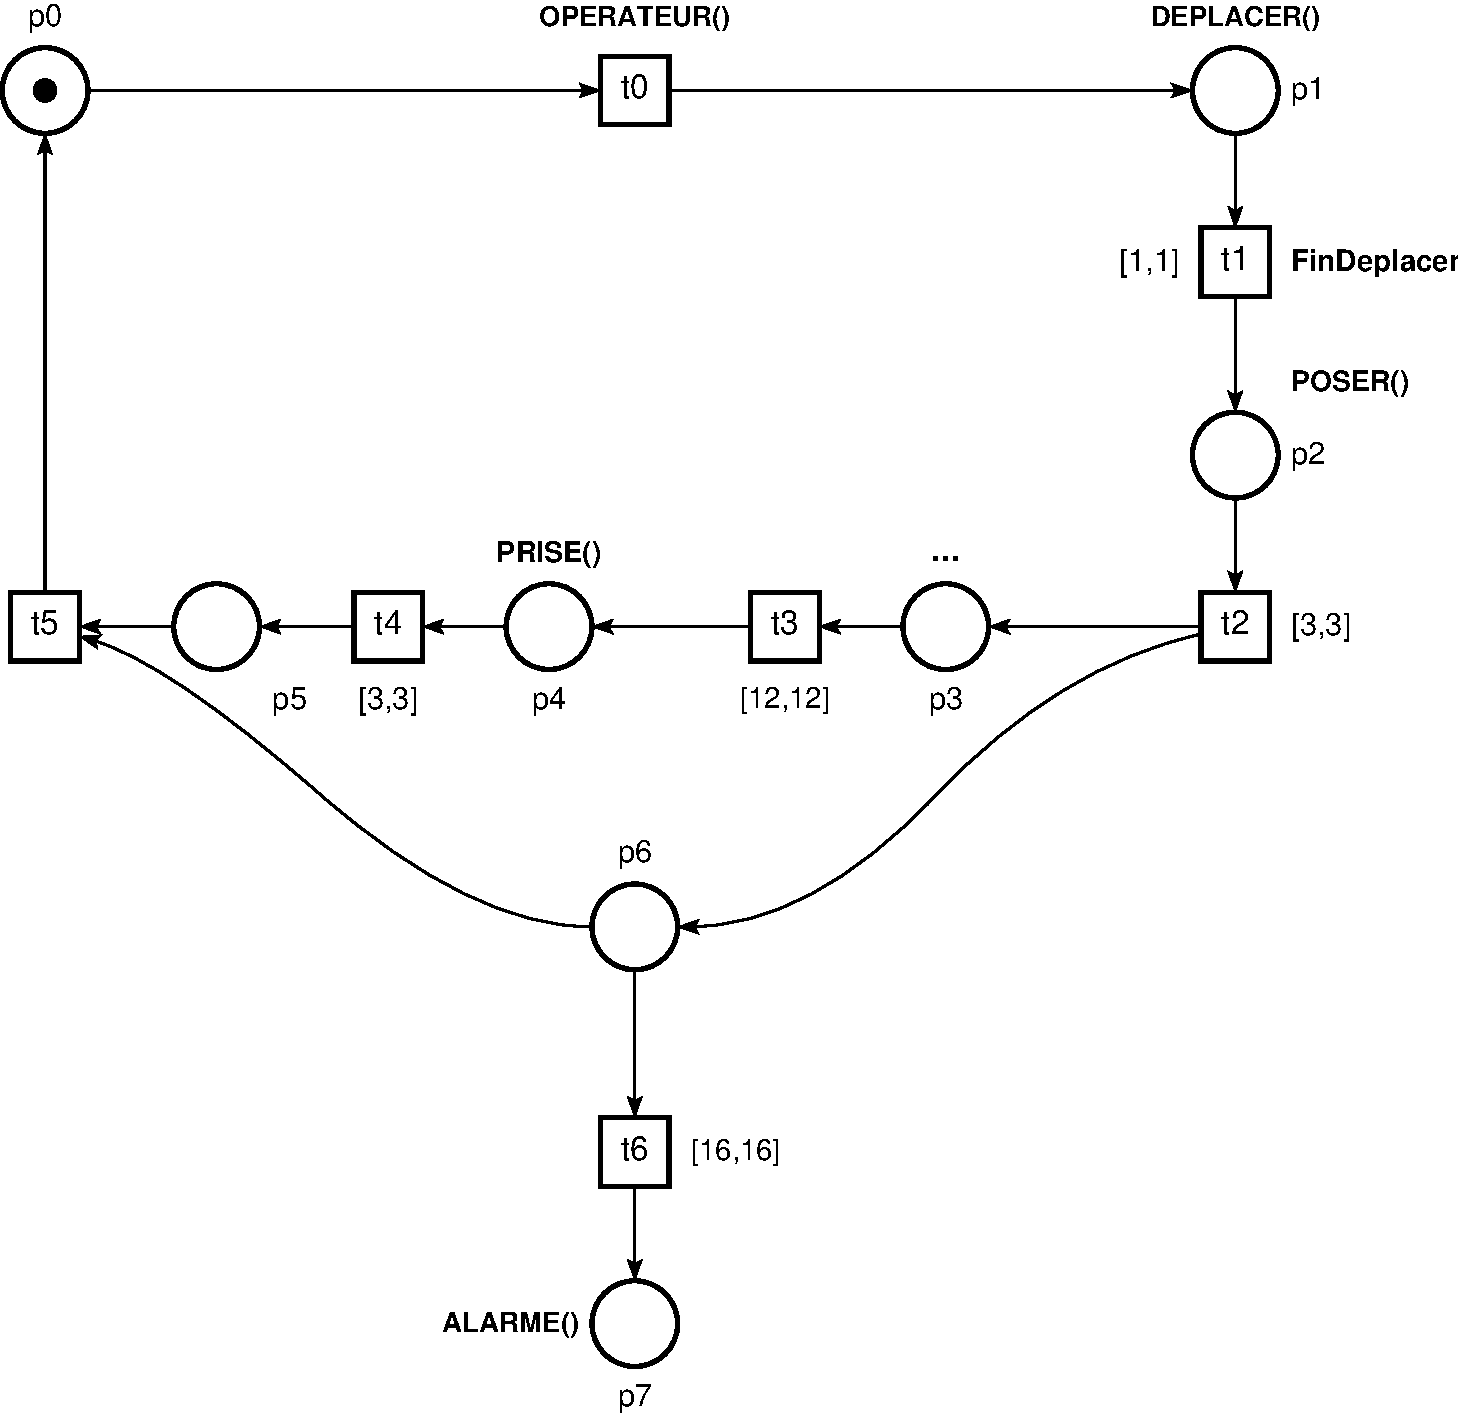
\includegraphics[width=.8\textwidth]{./I/images/III-1_v3_esti.pdf}
\caption{\label{fig:RdPTempo_generique_indentif}Modèle réseau de Petri générique d'une opération avec les temps estimés}
\end{minipage}\hfill%
\begin{minipage}[t]{.58\textwidth}
\centering
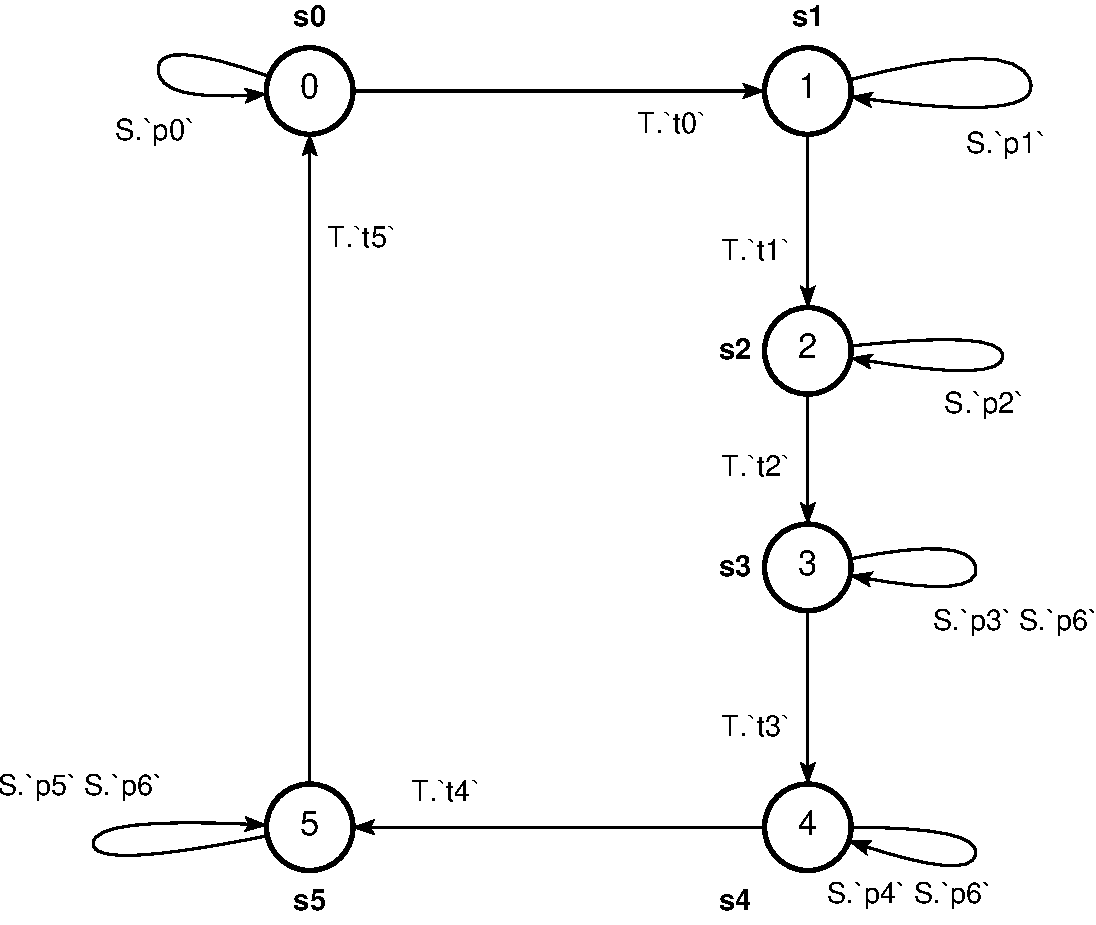
\includegraphics[width=.9\textwidth]{./I/images/III-1_v3_aut.pdf}
\caption{\label{fig:III-1-automate}Diagramme de classe.}
\end{minipage}
\end{figure}
Une analyse à l'aide de TINA nous a permis de déterminer les différentes classes du réseau. L'automate est présenté figure \ref{fig:III-1-automate}. Nous avons put aussi extraire les propriétés suivantes grâce à TINA.

\begin{itemize}
\item Le RdPT (Réseau de Petri Temporisé) n'est pas vivant. 
\item La transition $t_6$ est non vivante. 
\item LE RdPT est borné.
\end{itemize}



\chapter{Modélisation et analyse des premières opérations de chaque pièce}
Maintenant que nous connaissons un modèle valide pour une opération ainsi que les temps nécessaires au déplacement du chariot sur l'axe vertical et horizontal, nous allons pouvoir commencer à modéliser le travail du \emph{STA} sur deux opérations.

Nous allons, dans un premier temps, effectuer une modélisation en RdP Temporels d'une commande de deux opérations suite à quoi, nous en effectuerons une analyse grâce à une version de \emph{TINA} identique que dans le chapitre \ref{chap:realisationUneOperation}. Nous utiliserons cette analyse pour déterminer les intervalles d'attentes et le meilleur ordonnancement possible pour ne pas déclencher l'alarme.

\section{Réseau de PETRI Temporels de commande de deux opérations}
A partir du modèle générique établit en \ref{sec:modelGenerique}, nous avons obtenu, pour la commande de opérations $O_1$ et $O_2$ le modèle RdP Temporels en figure \ref{fig:command2Opes}.
\begin{figure}
\centering
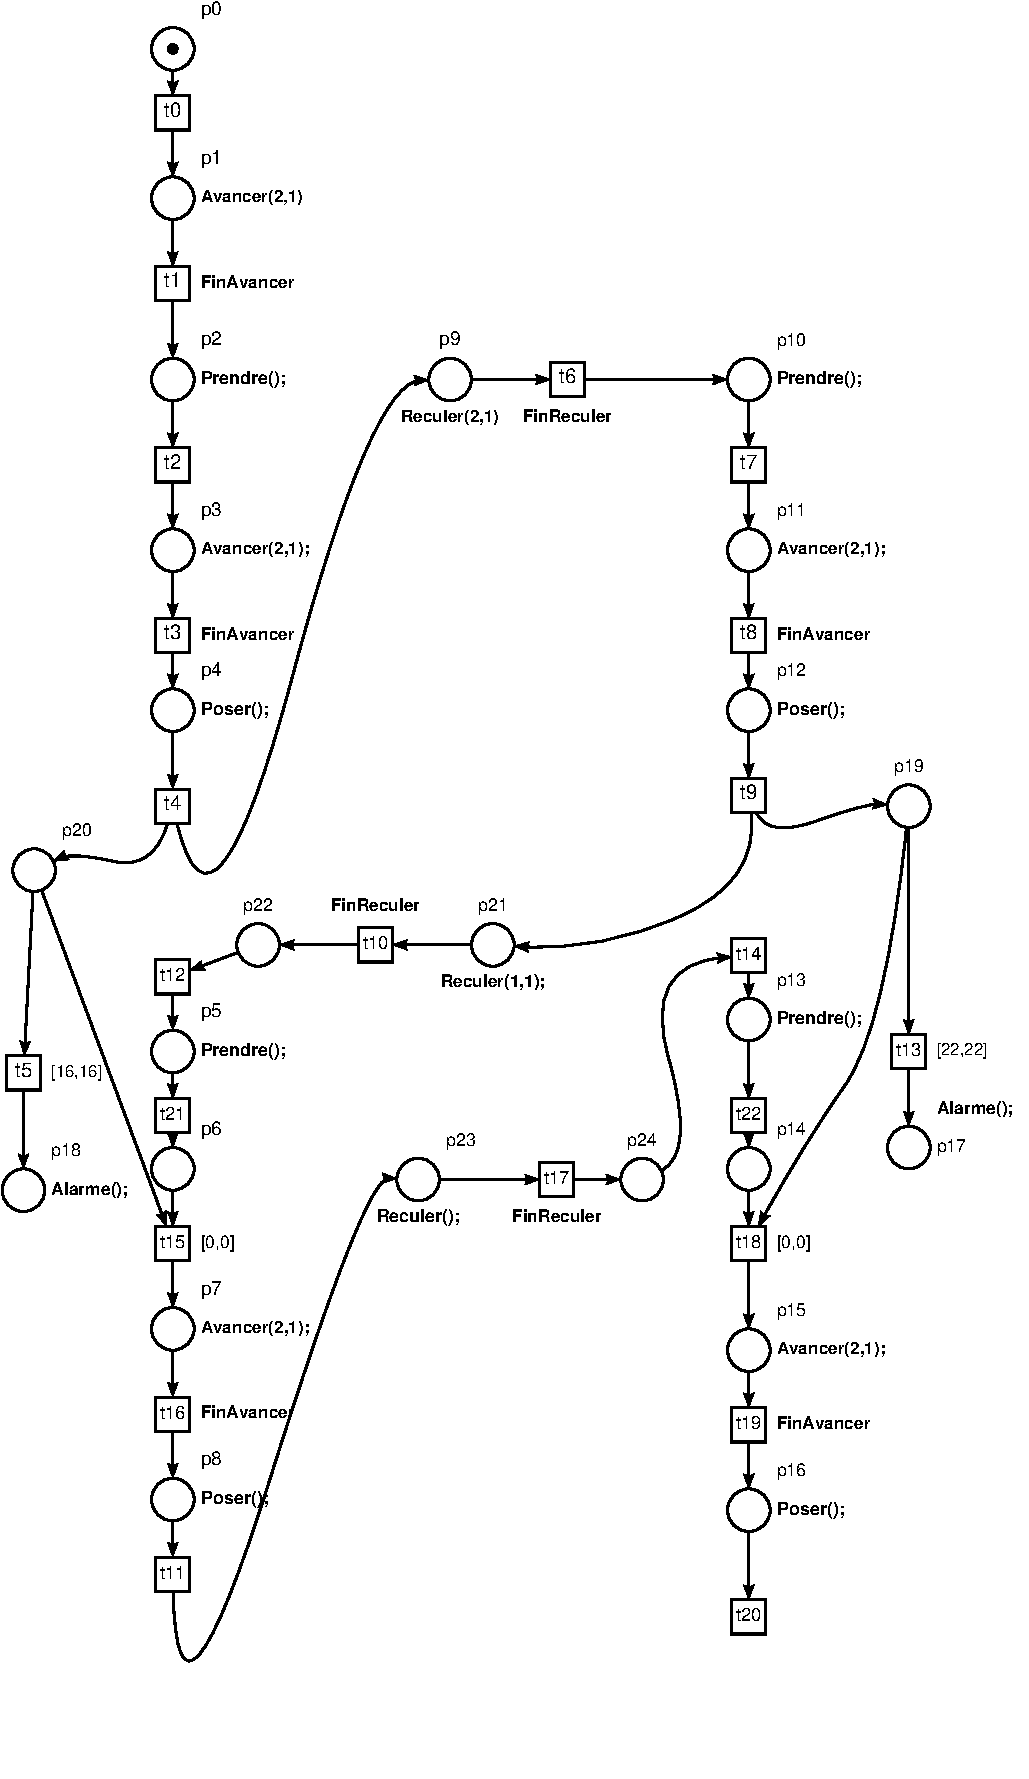
\includegraphics[height = \textheight]{./II/images/reseau_CommandeIII-2.pdf}
\caption{Réseau de PETRI Temporels pour la commande de 2 opérations}\label{fig:command2Opes}
\end{figure}

Dans ce réseau, nous pouvons identifier tout d'abord la ressemblance avec le modèle générique (en figure \ref{fig:RdPTempo_generique}) : les places $p_4$ et $p_{12}$ sont les représentations de la place $p_2$ dans le modèle générique. Elles seront donc suivi, dans les modèle Temporels que nous analyseront, d'une transition qui contient le temps des opérations \emph{Poser}. Il en va de même pour les places $p_2$, $p_{10}$, $p_{5}$ et $p_{13}$ qui contiennent l'opération \emph{Prendre}, elles seront suivi d'une transition contenant une intervalle de temps $y$.

\paragraph*{Séparation du modèle}
Nous pouvons séparer ce modèle complexe en deux ensembles de places : \begin{itemize}
\item l'ensemble $P_1 =\left\lbrace p_2,p_3,p_4,p_5,p_6,p_7,p_{20},p_{18}\right\rbrace$ est utilisé pour emmené la pièce $p1$ du bac $e1$(son bac initial) vers le bac $e3$ dans lequel elle subit l'opération $O_2$. Cet ensemble est lié avec les deux places $p_{20}$ et $p_{18}$ qui modélisent l'alarme liée à l'opération $O_1$.
\item  l'ensemble $P_2 =\left\lbrace p_{10}, p_{11}, p_{12} p_{13}, p_{14}, p_{15}, p_{16}\right\rbrace$ modélise le transport de la pièce $p2$ de $e2$(son bac initial) vers $e3$, bac dans lequel elle subit l'opération $O1$, puis du transport de $e5$ vers $e7$ (Pour prévoir les prochains RdP). L'alarme de l'opération est enclenchée par la place $p_{17}$, qui est lié au reste de l'ensemble $P_2$ par la place $p_{19}$.
\end{itemize}
	
\paragraph*{Liaison entre les ensembles}
Les places $p_9$, $p_{21}$ et $p_{23}$, places qui se situent entre les deux ensembles $P_1$ et $P_2$, sont utilisées pour effectuer les passages entre les 2 ensembles. De même, nous avons deux places $p_{22}$ et $p_{24}$ qui font la liaison entre les deux ensembles, à l'attention que celles ci ne servent pas à amener la chariot d'une pièce à l'autre mais à le faire attendre le temps nécessaire avant la fin d'une opération et donc la récupération d'une pièce.


Nous notons aussi les transitions $t_{15}$ et $t_{20}$ qui sont les représentations de la transition $t_5$ dans le modèle générique. Elles permettent dans ce contexte de synchroniser la prise de la pièce et l'arrêt du compteur de l'alarme. Comme dans le modèle générique, ces transitions ont un intervalle de temps $[0;0]$, cela oblige les jetons arrivant dans les places en amont à être immédiatement tiré. Ainsi, le compteur de l'alarme est stoppé après $0$u.t. que la pièce ait été retiré de son emplacement.

\paragraph*{Ordonnancement}
Il est aussi a noté que nous avons choisi d'effectuer l'opération de la pièce $p1$ avant celle de $p2$ et cela pour des raisons temporelles. Nous avons remarqué, dans une étude préliminaire à la construction de ce réseau, que cet ordonnancement était possible alors qu'une inversion l'ordre du traitement des pièces donne obligatoirement le retentissement d'une alarme (notamment dans la suite du TP).


Nous avons maintenant à notre disposition une commande à appliquer sur les \emph{STA}. Toutefois, avant de passer à l'implémentation, nous allons utiliser l'outil \emph{TINA} pour analyser le modèle ainsi obtenu.	


\section{Analyse du modèle avec TINA}
L'analyse temporelle de réseau nécessite un réseau tel que nous vous présentons en figure \ref{fig:RdpAnalyseIII-2}. Dans ce type de réseau, nous avons choisi de ne plus utiliser des noms sur les évènements mais plutôt des intervalles de temps. Ces intervalles ont été établi dans la section \ref{sec:estimationTemps}.

\begin{figure}[!ht]
\centering
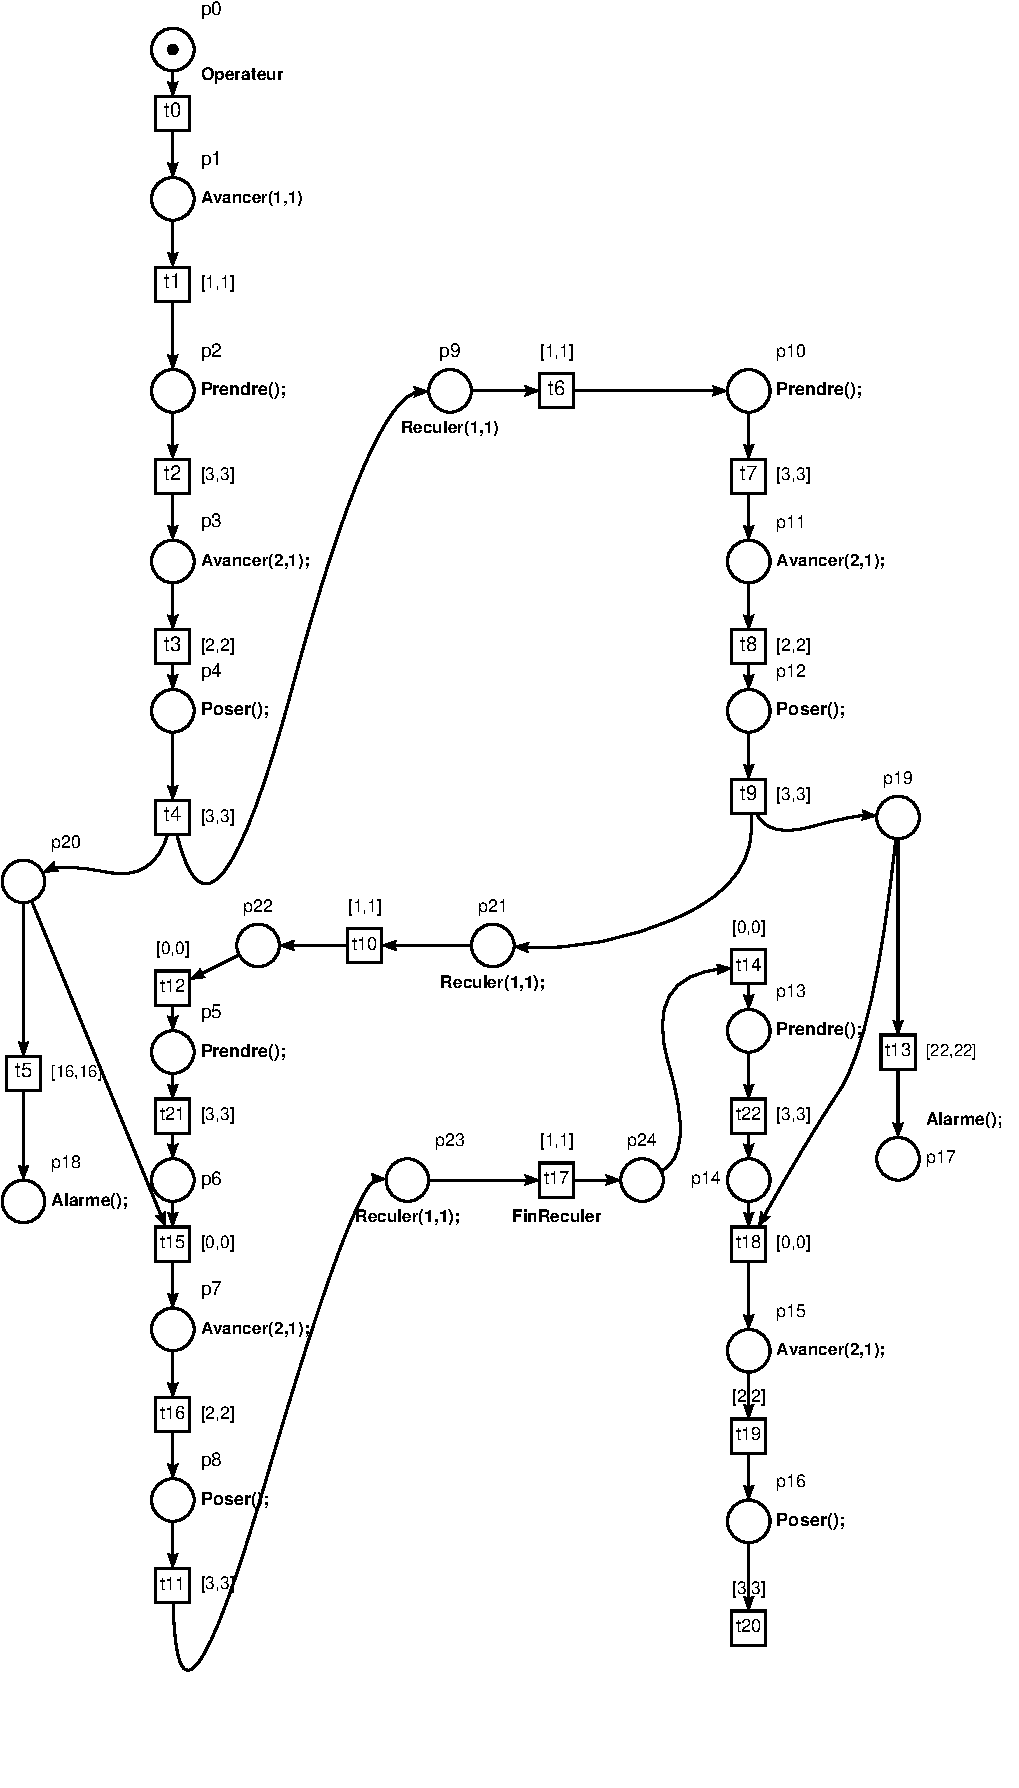
\includegraphics[height = .78\textheight]{./II/images/reseau-AnalyseIII-2.pdf}
\caption{Réseau de PETRI Temporels pour l'analyse de 2 opérations}\label{fig:RdpAnalyseIII-2}
\end{figure}

Avec la version de \emph{TINA} adéquate, nous avons réalisé la construction d'un graphe des classes accessibles. Ce graphe comporte 22 classes que nous n'avons pas représenté graphiquement, cependant vous pouvez trouver le rapport d'analyse du logiciel en annexe \ref{Annex:analyse}. 

\paragraph*{Vivacité du réseau} Dans cette analyse, nous nous referons dans un premier temps à cette bonne propriété. En effet, le résultat obtenu (disponible à la ligne 244) nous indique que les 2 transitions $t_5$ et $t_{13}$ ne sont jamais franchi. Ceci signifie que les places $p_{18}$ et $p_{17}$ ne sont jamais marqué, car le seul moyen existant pour qu'un jeton soit dans ces places est en franchissant respectivement cette transition. Donc, l'alarme n'est jamais activée.

\paragraph*{Graphe des classes}Une analyse des places accessibles à partir du graphe des classes nous confirme ce que la vivacité du réseau nous avait indiqué : les places $p_{18}$ et $p_{17}$ ne sont jamais marquées. 

Cette analyse nous apporte aussi une information que nous pourrons utiliser dans la prochaine section. Il s'agit de l'intervalle temporelle restante avant le franchissement des transitions $t_5$ et $t_{13}$ avec lequel il est possible de connaitre l'intervalle temporelle passée dans l'opération $O_1$ et $O_2$, respectivement. Nous pouvons observer aux lignes 153 et 194 ces intervalles, elles sont de $[3;3]$ pour $t_3$ et de $[9;9]$ pour $t_{13}$. 

\paragraph*{Intervalles de temps des opérations} Intéressons nous maintenant au temps d'exécution des opérations. En regardant les intervalles de temps que doivent respecter $O_1$ et $O_2$, nous pouvons connaitre le minimum et le maximum de temps admis pour les opérations. De plus, nous avons à notre disposition le temps passé dans les opérations à l'aide des transitions $t_3$ et $t_{13}$, en regardant dans le graphe des classes les intervalles de temps durant lesquelles elles peuvent être franchies. 

Donc, si l'intervalle temporelle des transitions atteint $d_{i_{max}} - d_{i_{min}}$u.t, alors la pièce doit être sorti du bac. Nous allons donc, dans la prochaine section, faire en sorte que les dernières intervalles temporelle atteinte pour $t_3$ et $t_{13}$ soit comprises entre : $[0;d_{i_{max}} - d_{i_{min}}]$.

%--> On sait le temps des opé min max
%--> On connait alors le temps des opé (dispo sur les intervalles restant de t13 et t9) 
%--> On doit obtenir le max-min sur les lignes 153 et 194

\section{Mise au point des Intervalles Temporelles}
Avec la conclusion précédente, nous avons pu déterminer l'ajustement nécessaire. Toutefois, nous ne pouvons pas caler toutes les intervalles d'un seul coup, nous devons les placer l'une après l'autre, dans l'ordre dans lequel les opérations sont lancées.

\paragraph*{Opération $O_1$}
A partir du graphe des classes établit à partir du modèle \ref{fig:RdpAnalyseIII-2}, nous avons le dernier intervalle temporelle atteint par la transition $t_5$ à la classe 12 du graphe disponible en annexe page \pageref{Annex:analyse} qui est :
\begin{equation}\label{eqn:intervalleTemporelleT5}
3 \Leftarrow t_5 \Leftarrow 3
\end{equation} 
Nous savons que pour cette opération, la différence entre la durée maximale $d_{max}$ et la durée minimale $d_{min}$ d'une opération, qui est : $d_{max} - d_{min} = 16-15 = 1$, nous savons que l'intervalle \ref{eqn:intervalleTemporelleT5} doit inférieure à $1$, sans atteindre $0$. De cette manière, nous pouvons assurer que la pièce est restée dans l'opération suffisamment longtemps et n'a pas fait sonner l'alarme. Pour obtenir ce résultat sur $t_5$, nous modifions l'intervalle temporelle de la transition $t_{12}$ de cette façon : 
\begin{equation}
t_{12} \in [0;0] \text{ devient : }t_{12} \in [2;2] 
\end{equation}


Une fois cette transition modifiée, nous avons retracé un graphe des classes à partir duquel nous pourrons ajuster l'opération suivante. Une partie de l'analyse d'accessibilité est disponible en annexe, page \pageref{Annex:GDC-miseauPointI-Ope1}.
\paragraph*{Opération}


 
$d_{1_{min}} = 15$
$d_{2_{min}} = 20$

\chapter{Modélisation des séquences d'opérations des deux pièces}
Dans cette partie, l'objet de l'étude se porte sur la réalisation de 6 opérations, 3 par pièces (les opérations $o_1 , o_3 , o_5$ pour $p_1$ et $o_2 , o_4 , o_6 $ pour $p_2$). Il faut, dans un premier temps, trouver une séquence optimale telle que toutes les opérations soient effectuées en un temps minimum sans déclencher l'alarme. Ensuite, nous devons réaliser une commande en réseau de Petri temporel pour effectuer les opérations puis l'analyser à l'aide d'un graphe des classes. Dans un dernier temps, nous avons réaliser la commande en langage C. 
\section{Analyse d'ordonnancement}
Nous avons décidé d'étudier l'ordonnancement optimal par un chronogramme car nous avons trouvé l'approche graphique plus intuitive au vu du faible nombre d'opérations. Nous avons réalisé cet ordonnancement sur Excel en prenant pour échelle \emph{une case égale une seconde}. Le chronogramme (figure \ref{fig:ordoExcel}) est coupé en trois parties pour des raisons de visibilité : une ligne est réservée aux opérations liées à la pièce $p_2$, une seconde aux actions du charriot et une dernière aux opérations de $p_1$.

\begin{figure}[!ht]
\centering
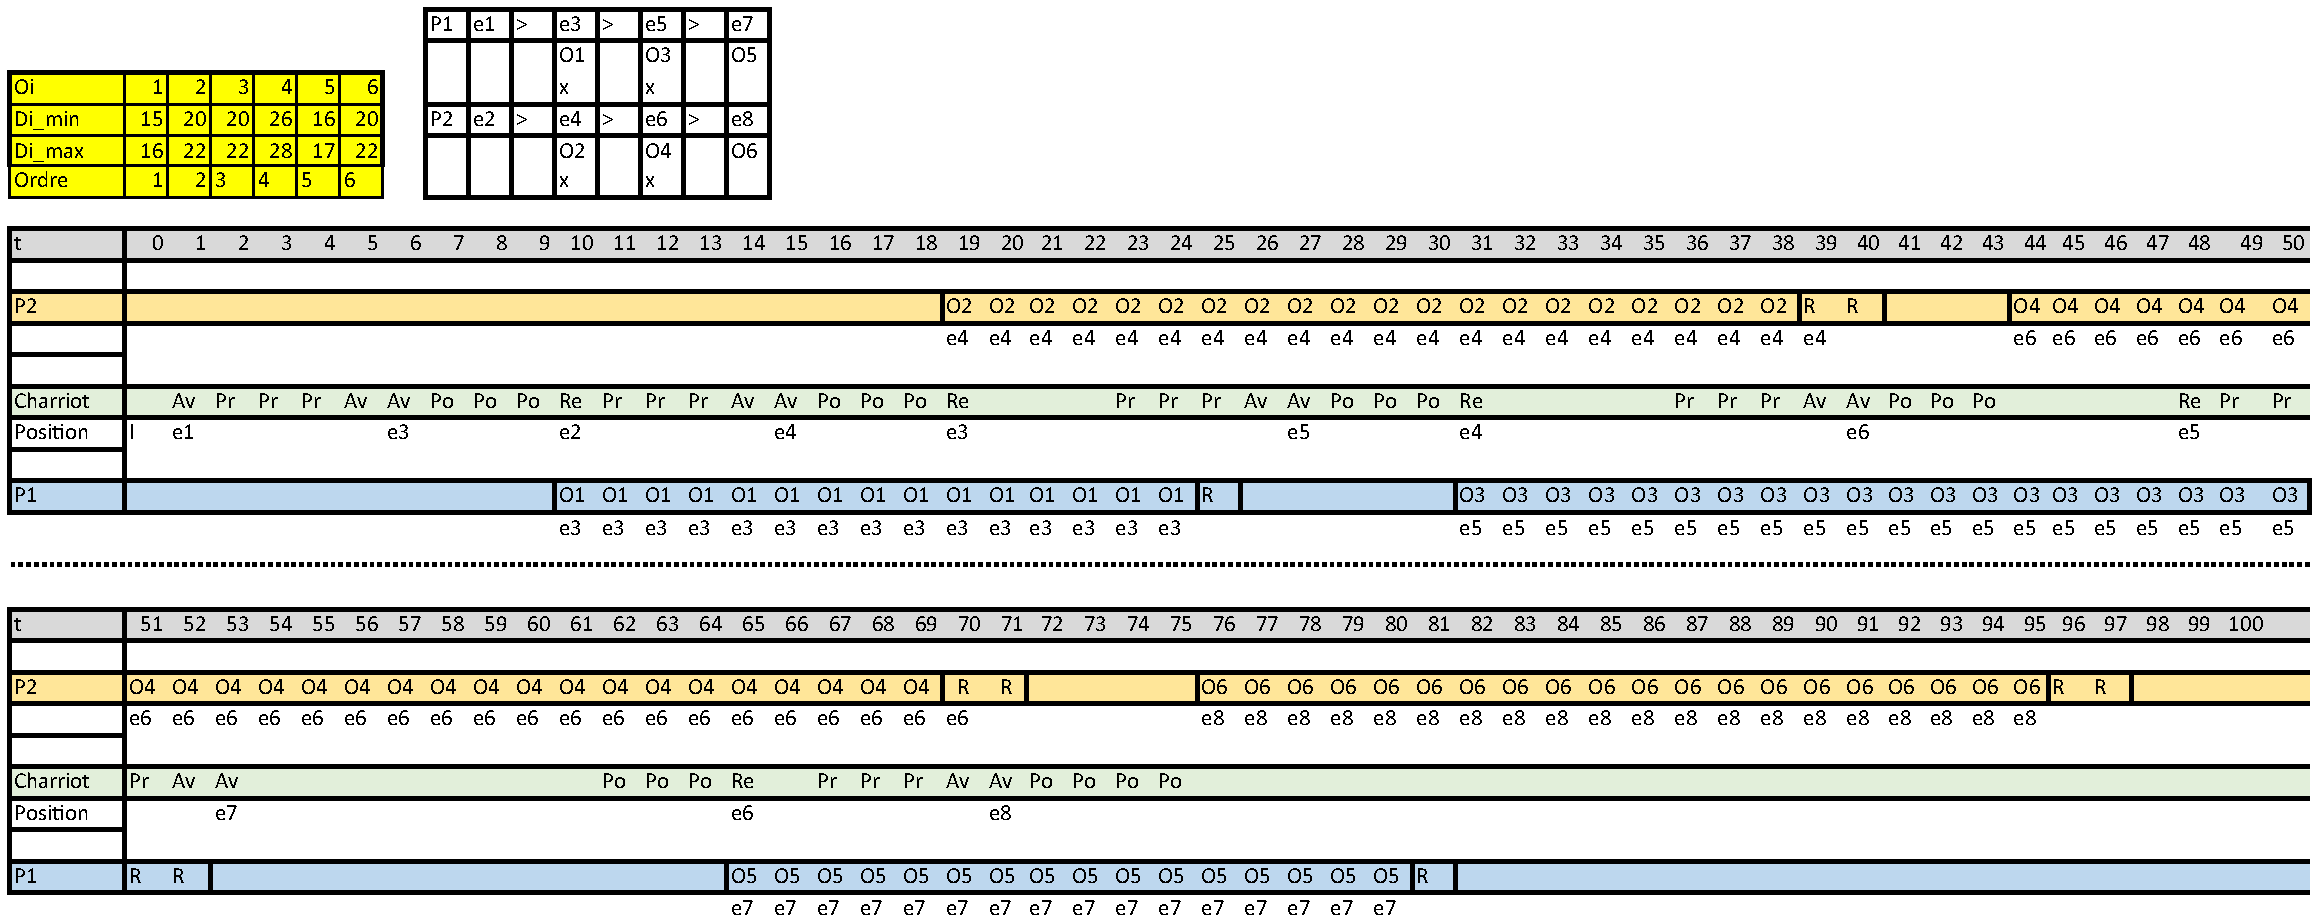
\includegraphics[width=\textwidth]{./III/images/ordo.pdf}
\caption{\label{fig:ordoExcel}Capture du tableur de calcul de l'ordonnancement.}
\end{figure}

Nous avons positionné les opérations au plus tôt, en vérifiant qu'elles n'empêchent pas de récupérer les pièces avant leurs alarmes respectives. Par exemple, l'opération $o_5$ pourrait commencer à partir de la 57\ieme seconde mais il serait impossible de retirer les deux pièces avant leurs alarmes donc nous avons décalé $o_5$ de façon à ce que, ni la pose, ni la prise de la pièce $p_1$ ne perturbe la prise et la pose de $p_2$. De plus, nous prenons pour hypothèse que les deux dernières opérations $o_5$ et $o_6$ n'ont pas de date récupération maximale et peuvent rester respectivement en $e_7$ et en $e_8$ car ces deux emplacements représentant le bac de sortie. Si nous avions pris le partie de les ramener à leurs emplacements initiaux, cela n'aurait pas été possible avec l'ordonnancement actuel, il aurait fallu organiser les opérations différemment de façon à avoir le temps de ramener les pièces au début ce qui nécessite beaucoup de temps à cause de la distance de déplacement importante.

\section{Réseau de Petri de commande}
Nous avons transformer la séquence d'actions de la ligne \emph{Chariot} de l'ordonnancement précédent (voir figure \ref{fig:ordoExcel}) en un réseau de Petri temporel. 
\section{Analyse par graphe de classes}

\section{Implémentation}

%\chapter{}



%\input{./V/chap5.tex}

%\input{./VI/chap6.tex}

%\input{./conclusions/conclusions.tex}

\chapter{Conclusion}

%Ne pas numéroter cette partie
\part*{Annexes}
%Rajouter la ligne "Annexes" dans le sommaire
\addcontentsline{toc}{part}{Annexes}
%\setcounter{chapter}{0}
\chapter*{Annexe 1 - Mesures des temps du Système physique}
\addcontentsline{toc}{chapter}{Mesures de temps}
\setcounter{section}{0}
% **********************************
%\addcontentsline{toc}{section}{TITRE}
\label{Annex:MesuresXY}
\lstdefinestyle{customc}{
%  language=C,                	  % choose the language of the code
%  numbers=left,                   % where to put the line-numbers
%  stepnumber=10,                   % the step between two line-numbers.
%  numbersep=5pt,                  % how far the line-numbers are from the code
%  backgroundcolor=\color{white},  % choose the background color. You must add \usepackage{color}
%  showspaces=false,               % show spaces adding particular underscores
%  showstringspaces=false,         % underline spaces within strings
%  showtabs=false,                 % show tabs within strings adding particular underscores
%  tabsize=2,                      % sets default tabsize to 2 spaces
%  captionpos=b,                   % sets the caption-position to bottom
%  breaklines=true,                % sets automatic line breaking
%  breakatwhitespace=true%,         % sets if automatic breaks should only happen at whitespace
%  title=\lstname,                 % show the filename of files included with \lstinputlisting;
  breaklines=true,
  frame=L,
  language=C,
  keywordstyle=\bfseries\color{green!40!black},
  commentstyle=\itshape\color{purple!40!black},
  identifierstyle=\color{blue},
  stringstyle=\color{orange},
  tabsize  = 2,
  showstringspaces=false,
}

\section{Mesure du temps de déplacement et de saisie/dépôt d'une pièce}
Dans le code suivant, vous trouverez le code des blocs FMG utilisé pour mesurer le temps de déplacement d'une case et de la prise du pièce. Nous avons pour cela implémenté la construction d'un Réseau de PETRI à 3 places : $p_0$ attend un appui sur "Opérateur", $p_1$ avance d'une case et $p_2$ prend une pièce. 

\lstinputlisting[title={Mesure de $x$, le temps pour avancer d'un emplacement et de $y$, le temps pour poser ou prendre une pièce.}, firstline =97, lastline = 179, style = customc]{./annexes/annexe1/mesureDesTempsPhysique_X.c} %{language = MAtlab}
\paragraph*{Résultat obtenu}Nous avons obtenu, à l'aide de ce code, l'affichage suivant:
\begin{itemize}
\item [\textbullet] "Avance  : $1.0$"
\item [\textbullet] "Prendre : $3.0$"
\end{itemize}

\section{Mesure du temps dedéplacement de bout en bout}\label{Annex:MesuresXY-boutEnBout}
\lstinputlisting[title={Mesure du temps de traversé de bout en bout.},
	firstline =97, 
	lastline = 165,
	style = customc]{./annexes/annexe1/mesureIntervalleTempsAvancerMaximal-clean.c} %{language = MAtlab}
	\paragraph*{Résultat obtenu}
	Pour compléter l'analyse des temps de parcours, nous avons étoffé nos résultats avec une dernière mesure : une mesure du point de départ du chariot jusqu'à la fin du rail.  Cette dernière mesure nous a semblé utile car nous avons remarqué que l'espacement des bacs n'était pas tout à fait identique. Avec le code disponible ci-dessus, nous obtenons un temps de traversé de bout en bout de $t = 9$, soit une seconde de plus. Étant donné que nous ne pouvons pas utiliser de décimale dans les intervalles temporelles du RdP, nous ne pouvons pas exploiter cette légère différence avec le temps $t=8$ attendu.
\chapter*{Annexe 2 - Analyse TINA}
\addcontentsline{toc}{chapter}{Analyse TINA}
\setcounter{section}{0}
\setcounter{subsection}{0}
% **********************************

\section{Analyse d'accessibilité du modèle 2 opérations}\label{Annex:analyse}
\lstset{title ={Analyse d'accessibilité du modèle 2 opérations, label = {lst:anal-2ope}},
		basicstyle = .5\footnotesize,
		numbers = left,
		stepnumber = 10}
\lstinputlisting{./annexes/annexe2/reseau-AnalyseIII-2-tina-W.txt}
	%


\newpage

%récupérer les citation avec "/footnotemark"
\nocite{*}

%%choix du style de la biblio
%\bibliographystyle{unsrt}
%%inclusion de la biblio
%\bibliography{bibliographie}
%%voir wiki pour plus d'information sur la syntaxe des entrées d'une bibliographie

\end{document}

